\scanpage{102}
\noindent 9) \uline{Application 1} L'isom.
$H^i(K,\unsure{\sigma|\gamma}_K)\longrightarrow\operatorname{Ext}^i_{k\text{-gr}}(J_{K/k},\unsure{\sigma|\gamma})$

\deleted{et le corps de classes de Serre}

(\unsure{Théorie} des corps de classes de Serre)

\margin{?\quad\figure{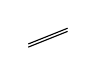
\begin{tikzpicture}\draw (0,0)--(.5,.2);\draw (0,-.04)--(.5,.16);\end{tikzpicture}}}
\noindent 10) \uline{Application 2} Autodualité de
\deleted{$\unsure{H^1}$}
$W_n(K)/F^mW_{\unsure{n}}(\unsure{K})$

\noindent 11) \uline{Application} 3 Cohomologie des V.A.

\noindent 12) L'isom de Lang \deleted{pour \unsure{un corps}}
\inserted{(sur corps $k$ fini)}

\noindent 13) \uline{Application} 4 Dualité de Tate.

\noindent 14) \uline{Compléments en égales caractéristiques}
\inserted{\uline{Théorie de Rosenlicht locale}}
\[
H^i(K,\unsure{\sigma|\gamma}_K)\simeq\operatorname{Ext}^i_{k\text{-gr}}(J_{K/k},\unsure{\sigma|\gamma})
\]
\margin{?}
pour $i>0$, tt $k$-groupe $\unsure{\sigma|\gamma}$, grâce à l'\unsure{isom}
canonique de $J(K)/J(V)'$.

\deleted{\[
\unsure{\mu_p\otimes\mu_p}\\
\unsure{\underline{\operatorname{Hom}}(\mu_p\otimes\mu_p,G_m)}
\unsure{\simeq}\unsure{\operatorname{Hom}(\mu_p,\mathbb Z/p\mathbb Z)}
\]}
\[
\left[\begin{array}{ll}
\uline{\text{Lang}}:&\text{\unsure{géom.} des corps de classes \unsure{prim.} globale par Rosenlicht + Lang}\\
\uline{\text{Serre}}:&\text{\unsure{géométrisation|généralisation} des corps de classes locale}\\
\uline{\text{Tate}}:&\text{Dualité de la cohomologie des V.A. sur un}\\
&\text{corps \unsure{p adique}.}
\end{array}\right.
\]
\mspage{101}

